\chapter{Referencial Teórico}
\label{CAP2}
\section{Ataques}
Ataques a uma rede de computadores sãos ações maliciosas em que \textit{softwares} são utilizados para de alguma forma prejudicar, interromper uma ação ou invadir uma rede ou máquina , afim de se beneficiar com tal ação. Todavia um ataque, deve ser caracterizado a partir de que se comprova que ele não é apenas ameaça e sim uma atividade maliciosa . Por isso, vale ressaltar que o ataque é a ação propriamente dita, enquanto, uma ameaça a um sistema é algo que possa afetar ou atingir o seu funcionamento, operação, disponibilidade e integridade. Podemos dizer que um ataque ocorre quando uma ameaça intencional é realizada \cite{dos2017ameaccas}.  Outra definição de ataque está relacionada com um tráfego não desejado, que é qualquer tipo de tráfego de rede não requisitado e/ou inesperado, cujo único propósito é consumir recursos computacionais da rede, desperdiçar tempo e dinheiro dos usuários e empresas e que pode gerar algum tipo de vantagem ou benefício (lucro) para seus criadores \cite{feitosa2008trafego}. 
\section{DoS}
Um dos tipos mais comuns de ataque é o DoS (Denial Of Service), que  é um tipo de ataque no qual se lança um grande número de requisições sobre uma vítima, de forma a sobrecarregar a vítima, evitando assim que a mesma faça algum tipo de trabalho "útil" \cite{handley2006internet}. Uma característica importante desses tipos de ataques é que o objetivo principal desse tipo de ataque não é a invasão em busca de dados ou informações, mas a negação do serviço que a vítima está utilizando ou oferecendo.  Uma das estratégias mais utilizadas para a realização desse tipo de ataque é o envio de múltiplas requisições à vítima em questão, de forma a gerar uma sobrecarga tal que ela não suporte tantas requisições e começe a negar serviços, o que fora da situação de ataque ela seria capaz de realizar normalmente\cite{mandia2001hackers}.

\section{DDoS}
DDoS (Distributed Denial of Service) é um tipo específico de ataque DoS de grandes dimensões, ou seja, que utiliza até milhares de computadores para atacar uma determinada máquina, distribuindo a ação entre elas \cite{alecrim2008ataques}. Trata-se de uma forma muito utilizada, já que é o tipo de ataque mais comum na internet. Esta é uma outra definição\: "Um ataque DDoS usa muitos computadores para lançar um ataque DoS coordenado contra um ou mais alvos. Usando a tecnologia cliente / servidor, o atacante é capaz de multiplicar a eficácia do DoS significativamente, aproveitando os recursos de vários computadores cúmplices involuntários, que servem como plataformas de ataque "\cite{stein2002world}.

\section{Detecção}
A detecção de um ataque DDoS é um trabalho relativamente complexo, uma vez que esse tipo de ataque ocorre em tempo real, e muitas vezes é difícil de ser identificado a máquina que é o atacante principal, por isso utilizamos o conceito de "tráfego não desejado". Como visto anteriormente, antes da ação do ataque acontecer, existem as ameaças aquela rede ou máquina, por isso tráfegos que não são desejados (que podem ser vistos como ameaça anteriormente a ação do ataque propriamente dito) devem ser identificados e o sistema de segurança podem tomar as devidas medidas. Existem muitas técnicas de detecção de ataques DDoS que fazem uso de cálculos estatísticos \cite{6814272}, porém essas soluções não proporcionam alta precisão de detecção DdoS, pois fazem uso de apenas um pequeno conjunto de recursos de tráfego, ou seja, com poucos dados de tráfego a detecção se torna inviável. A Correlação é uma medida estatística que é muito utilizada nas detecções de ataques \cite{yu2012discriminating}.

\section{Correlação}

Correlação é uma medida que mede o relacionamento entre duas variáveis .  Uma das maiores vantagens da correlação é que ela não necessita de uma grande quantidade de variáveis, para chegar a uma conclusão de relacionamento entre dois conjuntos. Portanto para uma detecção de ataques consistentes é necessária uma medida de correlação efetiva para classificar ataques DDoS  em tempo real, mesmo quando usa um pequeno número de recursos de tráfego. Uma correlação de forma resumida, é um conjunto de cálculos que, a partir das variáveis de entrada, retorna o relacionamento (similaridade, linearidade e direção) entre as variáveis, em um valor entre -1 e 1. Para calcular a correlação, é necessário se ter os valores de entrada, e um módulo (de \textit{software} ou \textit{hardware}) que realize os  cálculos abaixo descritos, retornando o resultado da correlação. Segue abaixo a fórmula da correlação, conhecida como NaHiD, implementada em hardware neste trabalho para detecção de ataques DDoS.

\begin{equation}
NaHiD(X,Y) = 1 - \frac{1}{n} \sum_{i=1}^{n} \frac{\left(|X(i) -	 Y(i)|\right)}{||\mu{X} - sX| - X(i)| + ||\mu{Y} - sY| - Y(i)|}
\end{equation}
onde
\begin{itemize}
	\item $\mu{X}$: Média aritmética do objeto de tráfego X.
	\item $\mu{X}$: Média aritmética do objeto de tráfego Y.
	\item $sX$: Desvio padrão do objeto de tráfego X.
	\item $sY$: Desvio Padrão do objeto de tráfego Y.
\end{itemize}

\section{Soluções em \textit{Hardware}}

Quando é necessário realizar um considerável número de cálculos em um dado sistema computacional, pode-se utilizar utilizar uma abordagem baseada em \textit{hardware}, em \textit{software} ou ainda uma abordagem mista. As utilizações de soluções baseadas em \textit{software} possuem duas grandes vantagens: Podem ser reutilizadas para soluções de propósitos gerais, além serem de fácil implementação. Já as soluções baseadas em \textit{hardware}, tendem a oferecer um alto desempenho e baixo consumo de energia \cite{HOQUE201748}.  Na abordagem de Ataques DDoS, utilizamos um sistema misto, baseado em \textit{hardware} e \textit{software}, para detectar, em tempo de acontecimento, os ataques. Precisa-se portanto de velocidade e precisão numérica suficiente para diferenciar ataques de situações normais. \textit{Softwares} contendo cálculos matemáticos complexos, em geral exigem grande quantidade de ciclos de CPU, o que pode implicar em uma detecção atrasada. Entretanto, uma arquiteturas baseada em solução mista, de hardware e software, pode oferecer o desempenho e precisão necessários, uma vez que tenhamos a flexibilidade de portabilidade do \textit{software}, e pelo lado do \textit{hardware}, ciclos de execução implementados de acordo com o problema específico \cite{miranda2002computador} .

\section{Técnicas Utilizadas}
Nota-se que a correlação proposta por \cite{HOQUE201748}, necessita de uma certa precisão, pois a mesma é uma medida de detecção. Para tal é necessário que os resultados de suas operações aritméticas tenham uma certa precisão. É  necessário estudar cada componente dessa formulação, e realizar a implementação em \textit{hardware} de forma que o sistema possa tirar conclusões assertivas, a partir de cálculos precisos. Serão descritas as operações e as formas em hardware de se realizar esses cálculos:

\subsection{Soma:} A soma pode ser implementada, com componentes do tipo somador aritmético, já bem conhecidos pela comunidade. Vale ressaltar que a soma pode ser utilizada no módulo, média e desvio padrão.
\subsection{Módulo:} O módulo pode ser facilmente implementado em \textit{hardware} com componentes do tipo somador. Vale ressaltar que o módulo pode ser utilizado no desvio padrão.
\subsection{Divisão:} A divisão de dois números quaisquer possui uma certa complexidade em \textit{hardware}, por não utilizar em suas operações apenas o conjunto dos números naturais, tendo que utilizar os conjuntos dos números fracionários. Para isso, utilizou-se um IP da plataforma VIVADO da \textit{Xinlix}, chamado \textit{Divider Generator}, esse IP realiza possui uma implementação de divisão de dois números, e retorna um resultado em uma representação de números fracionários com uma precisão escolhida de forma personalizada \textit{Divider Generator v5.1 LogiCORE IP Product Guide}. Um conjunto opções de configuração desse IP, implica em uma latência específica (quantos ciclos de clock, são necessários para um término de operação) da computação da de divisão. Uma dessas opções consiste justamente no uso de aritmética de ponto fixo, em particular na quantidade de bits utilizada para representar a parte inteira, assim como a parte fracionária.

\subsubsection{Aritmética de Ponto Fixo} 	

Para a representação de números fracionários, tem-se duas abordagens mais conhecidas: Ponto fixo e Ponto Flutuante. A representação em ponto flutuante trás consigo grande flexibilidade e precisão, porém a um custo muito elevado em termos de \textit{hardware}, adotando uma representação baseada em mantissa e expoente, requer circuitos de hardware com complexidade que vão muito além dos somadores aritméticos comuns de números naturais, que são os mesmos utilizados para aritmética de ponto fixo. A representação em ponto fixo divide a palavra binária em duas partes com quantidades de bits pré-determinadas(parte que representa o número inteiro e parte que representa em decimal), deixando portanto a precisão de ambas as partes sempre constante. A vantagem da representação em ponto fixo é facilidade e custo da implementação em \textit{hardware} frente a representação em ponto flutuante, gerando um excelente desempenho e uma certa precisão nos resultados \cite{woods2008reconfigurable}, desde de que se faça uma boa escolha da quantidade de bits a atribuir para cada uma das duas partes, o que requer um conhecimento prévio da faixa numérica a ser representada em cada parte (inteira e fracionária).

Na figura \ref{fp} podemos ver um exemplo de um número fracionário representado em ponto 4.4, ou seja, 4 bits representando a parte inteira e 4 bits representado a parte decimal. 

\begin{figure}[H]
	\centering
	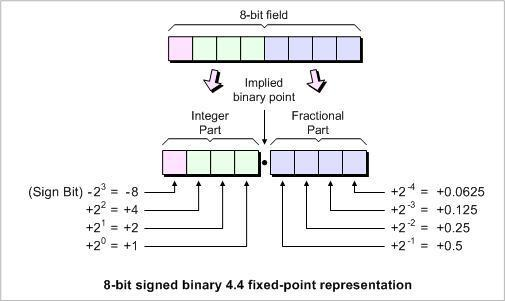
\includegraphics[width=8cm]{figures/fp.jpg}
	\caption{Representação de aritmética de ponto fixo}
	\label{fp}
\end{figure}




\subsection{Média aritmética:}  A média aritmética é um tipo de soma de variáveis seguido por uma divisão, sendo esta  última a parte mais complexa da média aritmética. Uma alternativa viável é utilizar divisão aritmética binária, de forma que, com pequenos ajustes em uma operação (ajustes que não influenciem no resultado dessa operação), seja gerado um resultado aproximado. No caso da média , seriam uma operação de soma de todos os elementos em questão, dividido pelo número de elementos, segundo {4} a divisão por números pares são aproximadas do resultado apenas pelo deslocamento de algum bit, desprezando a parte fracionária. Vale ressaltar que a Média Aritmética pode ser utilizada no desvio padrão.

\subsection {Desvio padrão:} O Desvio padrão é a variável em questão subtraída da média, após isso elevada ao quadrado. Após essa série de cálculos, calcula-se a raiz quadrada, tendo então o desvio padrão. Então é necessário um multiplicador para realizar essa potenciação, bem como um módulo calculador de raiz quadrada. Multiplicadores são facilmente encontrados implementados em silício nas FPGAs. Já a raiz quadrada, por ser um cálculo mais específico, requer a utilização de um IP core que faça o calculo. Para isso pode-se utilizar um  IP da plataforma VIVADO da Xinlix, chamado CORDIC {CORDIC v6.0} , que realiza  implementação de cálculo de raiz quadrada. Basicamente esse IP recebe uma variável como entrada, e em sua saída retorna a raiz quadrada aproximada do número de entrada. A configuração das opções dsse IP implica em uma certa latência (quantos ciclos de clock, são necessários para um termino de operação) da computação.



\section{FPGA}
Quanto mais se conhece a respeito do problema a ser resolvido, mais acertada será a escolha de que tipo de abordagem se deve utilizar, para acomodar a lógica do problema em questão. Como foi pontuado acima, o problema da detecção de ataques em tempo real, requer duas características principais, desempenho e precisão. Para realizar essa detecção poderíamos utilizar dois tipos de unidade de processamento mais conhecidas ASICs(Circutos integrados para uma aplicação específica) e as FPGAS(Arranjo de Portas Programáveis em Campo). Porém segundo \citeonline{HOQUE201748}, as FPGAs oferecem adaptabilidade dinâmica, que é importante para aplicações que requerem mudanças frequentes em suas configurações, como a detecção de ataques DDoS que evoluem com freqüência. Além disso segundo \citeonline{heath2002embedded} O tempo de projetos baseados em FPGA é normalmente conhecido com muita precisão a priori, o que trás um certo conforto para a equipe de projeto.




\section{FPGA'S Xinlix de série 7}
As FPGAs da série Xilinx 7 compreendem quatro famílias de FPGA que abordam uma gama completa de requisitos nos sistemas como: baixo custo, pequenos tamanhos, sensíveis ao custo, aplicações de alto volume de largura para altas conectividades, capacidade lógica e capacidade de processamento de sinal para aplicações de alto desempenho \cite{przybus2010xilinx}.

Artix (Baixo custo) , Kintex (Balanço de alta performance com baixo custo), Virtex (Sistemas de alta performance) e ZYNQ (Aplicações em sistemas embarcados em geral).
A diferença entre essas famílias está basicamente em sua performance e baixo consumo , consequentemente para qual finalidade elas deverão ser usadas, vale ressaltar que custo e energia está diretamente ligado a baixo consumo de potência como podemos ver na Figura \ref{comparative}. Pra corroborar com isso nota-se que cada família tem variações em relação máxima capacidade dos recursos que ambas possuem, como Células Lógicas, Blocos de RAM , pinos E/S e etc .
Cada bloco lógico configurável (CLB) é composto por dois \textit{Slices} que podem ser do tipo M (SLICEM) , podem ser utilizados para memória e lógica, ou do tipo L (SLICEL), podem ser utilizados apenas para lógica e aritmética. 
Cada \textit{Slice} pode ter como recursos gerenciáveis 4 LUTs(Look-up Tables) de 6 entradas , multiplexadores , \textit{carry chains} e 4 flip-flops/latches.
As interfaces E/S, em geral, trabalham pra proporcionar altas velocidades de resposta sem tentar perder integridade no sinal. Além de serem projetadas para diferentes padrões (Voltagens, larguras e protocolos). Nas famílias da 7 series elas podem ser caracterizados por dois tipos : High Range (HR), suportando padrões I/O de tensões de ate 3.3 V,  e High Performance (HP), suportando somente padrões I/O de tensões de até 1.8V e projetado para alta performance, por isso dependente da família.
Todos os membros das famílias de série 7 tem o mesmo bloco \textit{RAM/FIFO(First in first out)} , operação totalmente síncrona, muitas opções de configurações \textit{(true dual port, simple dual-port, single-port)} e etc \cite{demetrioarquitetura}. 

\begin{figure}[H]
	\centering
	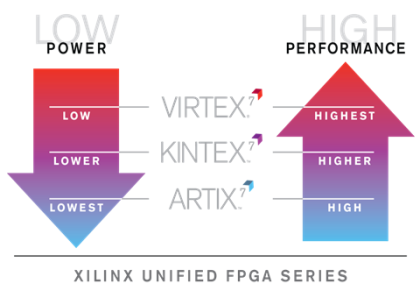
\includegraphics[width=8cm]{figures/xi-lite-01.png}
	\caption{Comparativo de potência e perfomance entre as famílias da série 7 da Xilinx}
	\label{comparative}
\end{figure}
